% document.tex
% This is the root of the document for my boilerplate lab report.
% Author: Dennis Ogbe, dogbe@purdue.edu

\documentclass[12pt]{article}
\usepackage{boilerp} % all of the formatting info is in ./boilerp.sty

% Bibliography file 'references.bib' in working directory
\bibliography{references}
\nocite{*} % show all of the references, even when not used

% Page header & footer
\pagestyle{fancy}
\fancyhead[LH]{Project: Generator Excitation Control} % left header
\rhead{ECE 4210 Control System Design I, Fall 2013} % right header
\fancyfoot[CF]{\thepage}

\begin{document}

% the title page
  % title.tex
% Author: Dennis Ogbe
%
% This is a template for a title page for reports in class.
% copy/ paste this code to the top of your documents
% and don't forget to add the following line at the top
% of each document:
% "\newcommand{\HRule}{\rule{\linewidth}{0.4pt}}"
%
% Also, don't forget to add the file
% "PU_signature_KOG_cmyk_Reg.eps" from this directory
% to the directory of your document
%
% to compile this example title page, take a look at
% "test_title.tex"

\begin{titlepage}
\begin{center}
\thispagestyle{empty}
\vspace*{2.5cm}

\Huge
\HRule \\
\vspace{0.5cm}
\textbf{This is my Title.}\\
\HRule \\

\vspace{0.1cm}
\large
This is my subtitle\\
\normalsize
\vspace{1.5cm}
Author: Dennis Ogbe
\\
\vspace{0.5cm}
Class: ECE 6666 Black Magic Design Research, Winter 2054
\\
\vspace{0.5cm}
Due Date: September 13, 2013

\vspace{4.5cm}


\includegraphics[scale=0.8]{./title/PU_signature_KOG_cmyk_Reg.eps}\\
\vspace*{0.5cm}
School of Electrical and Computer Engineering\\
\vspace{0.5cm}
Purdue University


\end{center}
\end{titlepage}
\setcounter{page}{2}


% table of contents etc.
\newpage
\tableofcontents
\newpage
% \listoffigures
% \newpage
% \listoftables
% \newpage

% include the different sections here. every section should go into its own file.
  \section{Abstract}
The following is a project report describing the excitation control of a 5 kV generator system. It will cover background information on generator systems, the modeling of a generator system, the control of a generator system using negative feedback control systems, and the design of a compensator to meet required specifications set by the designers.



  \section{Backround}
The invention of generators was made possible by Michael Faraday's discovery of electromagnetic induction in 1831 \cite{faraday}. Faraday was able to demonstrate his discovery with a simple generator, however, there was little need for the production of electricity at that point in time. Nikola Tesla invented the first polyphase AC generator which superimposed several different AC flows into a single polyphase output. With a practical AC generator in hand, along with transformers to raise and lower voltage, Tesla's system could be used to implement large distribution networks. These larger systems, such as the Niagara Falls hydroelectric plant built in the 1890s, lower costs and paved the way for power systems as we know them today \cite{generators}.



  \section{Introduction}
One of the most important components of power systems is the three-phase synchronous generator or alternator. Synchronous generators have two synchronously rotating fields. One field is produced by the rotor driven at synchronous speed and excited by DC current, and the other field is produced in the stator windings by the three-phase armature currents. The DC current for the rotor windings is produced is provided by the excitation systems. In older units, the exciters are DC generators mounted on the same shaft, providing excitation through slip rings. Today's systems use AC generators with rotating rectifiers, known as brushless excitation systems. The generator excitation system maintains generator voltage and controls the reactive power flow. Because they lack the commutator, AC generators can generate high power at high voltage, typically 30 kV. In a power plant, the size of generators can vary from 50 MW to 1500 MW. Steam turbines operate at relatively high speeds of 3600 or 1800 rpm for 60Hz operation. In a power system, several generators are operated in parallel in the power grid to provide the total power needed \cite{analysis}.

Loads of power systems are divided into industrial, commercial, and residential. Industrial loads are functions of voltage and frequency. They represent a large portion of system load due to the large number of induction motors that consume a large amount of reactive power. Commercial and residential loads consist largely of lighting, heating, and cooling. These loads are almost entirely resistive and consume extremely small amounts of reactive power. The magnitude of these three combined loads varies dramatically throughout the day. Power must be made available to consumers upon demand, therefore, an advanced control system in necessary to properly supply the amount of power needed by consumers \cite{analysis}.



  \section{Characteristics of a Generator System}
Synchronous generators or alternators are synchronous machines used to convert mechanical power to AC electrical power. A DC current is applied to the rotor winding, which produces a rotor magnetic field. The rotor of the generator is then turned by a prime mover, producing a rotating magnetic field within the machine. This rotating magnetic field induces a three-phase set of voltages within the stator windings of the generator \cite{machinery}.

The rotor of a synchronous machine is a large electromagnet. The magnetic poles can be either salient or non-salient construction. Two common approaches used to supply a DC current to the field circuits on the rotating rotor. The first method is to supply the DC power from an external DC source to the rotor by means of slip rings and brushes. The second method is to supply the DC power from a special DC power source mounted directly on the shaft of the machine \cite{machinery}.

By definition, synchronous generators produce electricity whose frequency is synchronized with the mechanical rotational speed. The rate of rotation of the magnetic fields in the machine is related to the stator electrical frequency by Equation \eqref{eq:1} \cite{machinery}:

\begin{equation}\label{eq:1}
f_e = \frac{n_m P}{120}
\end{equation}

Where \begin{math}f_e\end{math} is the electrical frequency in Hz, \begin{math}n_m\end{math} is the mechanical speed of magnetic field, in r/min, and P is the number of poles. Equation (1) shows that 60 Hz power can be produced by rotating the shaft at 3600 r/min for a 2-pole machine and at 1800 r/min for a 4-pole machine.

The peak voltage produced by the generator is represented by Equation \eqref{eq:2} \cite{machinery}:

\begin{equation}\label{eq:2}
E_{max} = N_c\Phi\omega_m
\end{equation}

The RMS voltage is represented by Equation \eqref{eq:3}:

\begin{equation}\label{eq:3}
E_{A} = K\Phi\omega
\end{equation}

Where \begin{math}K\end{math} is a constant representing the construction of the machine, \begin{math}\Phi\end{math} is flux, and \begin{math}\omega\end{math} is rotation speed.

The internal generated voltage \begin{math}E_A\end{math} is directly proportional to the flux and to the speed, but the flux itself depends on the current flowing in the rotor field circuit. The voltage in a single phase of a synchronous machine is not usually the voltage appearing at its terminals. It equals the output voltage \begin{math}V_\Phi\end{math} only when there is no armature current in the machine. This is due to distortion of the air-gap magnetic field caused by the current flowing in the stator, self-inductance of the armature coils, and the resistance of the armature coils \cite{machinery}.

The phase voltage of a synchronous generator is given by Equation \eqref{eq:4} \cite{machinery}:

\begin{equation}\label{eq:4}
V_\varphi = E_A - jX_s I_A - R_A I_A
\end{equation}

where \begin{math}X_s\end{math} represents the armature reaction effects and the self-inductance in the machine. It is customary to combine them into a single reactance called the synchronous reactance of the machine \cite{machinery}:

\begin{equation}\label{eq:5}
X_s = X + X_A
\end{equation}

The terminal voltage \begin{math}V_T\end{math} will be \begin{math}\sqrt{3} V_\varphi\end{math} for a Y connected synchronous generator and remain \begin{math}V_\varphi\end{math} for a delta connected synchronous generator.

Three quantities must be determined in order to correctly describe the generator model. They are as follows: The relationship between field current and flux, the synchronous reactance, and the armature resistance. The behavior of a synchronous generator varies under load depending on the power factor of the load and on whether the generator is working alone or in parallel with other synchronous generators. Our system will have a sole synchronous generator operating alone. An increase in the load is an increase in the real and reactive power drawn from the generator. When a load is added the phase and terminal voltage for lagging, inductive loads decreases significantly. For purely resistive, unity power factor loads the phase and terminal voltage decreases slightly. For leading, capacitive loads, the phase and terminal voltage rises. The effects of adding loads can be described by the voltage regulation \cite{machinery}:

\begin{equation}\label{eq:6}
VR = \frac{V_{nl}-V_{fl}}{V_{fl}} 100\%
\end{equation}

Where \begin{math}V_{nl}\end{math} is the no load voltage of the generator and \begin{math}V_{fl}\end{math} is its full load voltage.

A synchronous generator operating at a lagging power factor has a fairly large positive voltage regulation while a synchronous generator operating at a leading power factor often has a negative voltage regulation. A synchronous generator operating at a unity power factor has a small positive voltage regulation. Because a constant terminal voltage supplied by a generator is desired and the armature reactance cannot be controlled, the terminal voltage can be controlled using the internal generated voltage,\begin{math} E_A=K\varphi\omega\end{math}. This is done by changing flux in the machine while varying the value of the field resistance, \begin{math}R_F\end{math}. Decreasing the field resistance 	increases the field current in the generator. An increase in the field current increases the flux in the machine. An increased flux leads to the increase in the internal generated voltage. An increase in the internal generated voltage increases the terminal voltage of the generator \cite{machinery}.

The real output power of the synchronous generator is:

\begin{equation}\label{eq:7}
P_{out} = \sqrt{3}V_T I_L \cos\theta = 3V_\varphi I_A \cos\theta
\end{equation}

The reactive output power of the synchronous generator is \cite{machinery}:

\begin{equation}\label{eq:8}
Q_{out} = \sqrt{3} V_T I_L \sin\theta = 3V_\varphi I_A \sin\theta
\end{equation}

In real synchronous machines of any size, the armature resistance \begin{math}R_A <<  X_s\end{math}, therefore, the armature resistance can be ignored. Thus a simplified phasor diagram indicates that \cite{machinery}

\begin{equation}\label{eq:9}
I_A \cos\theta = \frac{E_A \sin\delta}{X_s}
\end{equation}

Then the real output power of the synchronous generator can be approximated as \cite{machinery}

\begin{equation}\label{eq:10}
P_{out} = \frac{3 V_\varphi E_A \sin\delta}{X_s}
\end{equation}

Here \begin{math}\delta\end{math} is the torque angle of the machine, the angle between \begin{math}V_\varphi\end{math}  and \begin{math}E_A\end{math}.



  \section{Instrumentation}
Instrumentation is "the art and science of measurement and control" \cite{heitkamp}. In the scope of electrical control systems, instrumentation is the part of a system that measures the quantity that is to be controlled and that provides feedback about the value of that quantity to the control system. In most cases, the instrument of choice for a control system is some kind of sensor. Sensors come in many different varieties like temperature sensors, humidity sensors, altimeters etc. Since electrical control systems work with electrical signals, a sensor must be combined with a transducer that produces an electric signal relative to the measured quantity.

The quantity that is to be measured and controlled in this project is the terminal voltage of the generator. The instrument of choice in this case needs to able to measure the voltage of an electric signal and output a signal relative to that voltage. This device is called a "voltage transducer". The voltage transducer is at its core a voltmeter, but instead of providing the output on a numeric display, the output is an electrical signal that can be used in a control loop \cite{systematic}. Since the control system were to be implemented using the LabVIEW softwar, we use a I/O module that contains voltage transducers for use on a general-purpose computer \cite{labview}.



  \section{Modeling}
A model is a mathematical representation of a system that is determined by applying physical laws to a system and producing an equation.  The purpose of a model is to cut costs on the design because it is much less expensive to analyze an equation rather than a physical through trial and error.

An analytical model is created by determining the inputs and outputs of the system, which would include any type of signals going into the generator system and the effects the input has on the load.  Then, equations are developed based on known equations that represent the system.  Next, a transfer function is formed using the Laplace transform of the output of the system over the input.  This process is repeated for every input and output of the system.  From this model, critical system characteristics such as stability, accuracy, and speed can be optimized.  It is a good start seeing if a model will work in the real world with the transfer function \cite{analysis}.

An experimental model can be determined by collecting data output from a unit step input. This method produces more stable results because analytical models are based on ideal characteristics that are not entirely accurate for a real system. However, an experimental model has a higher cost due to expenses incurred for an accurate experiment. A typical design process would be to create an analytical model first, and then determine an experimental model in order to compare both models.

To obtain an accurate model for the generator system, a sequence of step response tests was performed, starting with an excitation voltage of 0.5 V and ending with a voltage of  5.0 V with increments of 0.5 V. It was observed that excitation voltages in the range from 1.5 V to 2.5 V produced terminal voltages in the desired range of 110 V. Figure \ref{fig:test_data} shows the results of the several step response tests.

\begin{figure}[h!]
\begin{center}
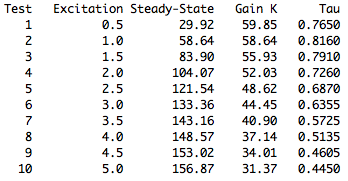
\includegraphics[scale=0.9]{./img/test_results.png}
\end{center}
\caption{Results of the step response tests}
\label{fig:test_data}
\end{figure}

One can obtain a first order transfer function model from the values of \begin{math}K\end{math} and \begin{math}\tau\end{math}. The equation for this model can be seen in eqn. \eqref{eq:tf_equation}:
\begin{equation}\label{eq:tf_equation}
G(s) = \frac{K}{1+\tau s}
\end{equation}

The modeled step responses were plotted and compared to the acquired data. Figure \ref{fig:model} shows an example plot of the recorded data and the calculated model for a excitation voltage of 2 V.
\begin{figure}[h!]
\begin{center}
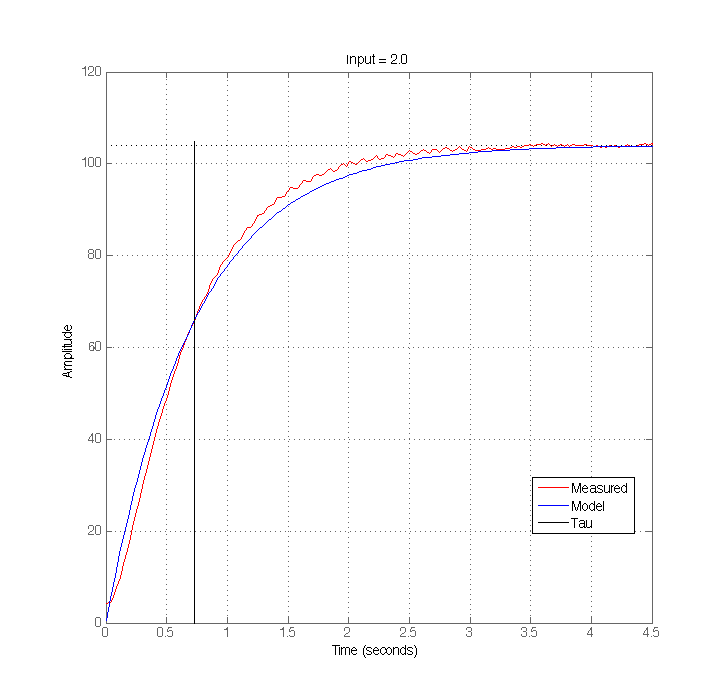
\includegraphics[scale=0.4]{./img/model.png}
\end{center}
\caption{Results of the step response tests}
\label{fig:model}
\end{figure}

We obtained our model by taking the arithmetic mean of the \begin{math}K\end{math} and \begin{math}\tau\end{math} values of the results of tests 3, 4, and 5. The resulting transfer function was:
\begin{equation}\label{eq:tf_model}
G(s) = \frac{52.19}{1+0.7347 s}
\end{equation}



  \section{Control}
In this project, the quantity to be controlled is the terminal voltage of the generator. The terminal voltage depends on the internally generated voltage \cite{machinery}. Since the rotation speed of the generator is kept constant, the only way to control the internally generated voltage is by controlling the strength of the rotor magnetic field, which, in turn, is dependent on the excitation voltage.
Therefore, the input to our control system is the DC excitation voltage that directly controls the output of the system, which is the terminal voltage.

The control system must be designed for the following scenario: The load on the generator output varies as the connected utilities are turned on and off. When the load changes, the terminal voltage on the generator changes as well \cite{machinery}. For the mostly resistive residential loads, this means that every time a heater or a light gets turned on, there will be a voltage drop in the terminal voltage. Since it is desirable to provide a constant voltage to customers, this voltage drop needs to be compensated quickly by an excitation control system \cite{modern}.

\begin{figure}[h!]
\begin{center}
\includegraphics[scale=0.7]{./img/figure.pdf}
\end{center}
\caption{Feedback Control System for Excitation Control}
\label{fig:sys}
\end{figure}

The control system needs to be a closed-loop feedback control system, with a voltage transducer as a sensor \cite{modern}. In order to minimize the drop in terminal voltage and to speed up the overall response of the generator, a compensator system will have to be designed \cite{modern}. The overall block diagram of the control loop is provided in Figure \ref{fig:sys}.

The voltage transducer measures the terminal voltage and provides feedback to the circuit.  The compensator stabilizes and speeds up the loop and provides the input voltage to the exciter. The exciter creates the magnetic field on the rotor, which determines the terminal voltage.

In order to control the generator at peak performance, a steady-state error of zero was needed, along with a fast settling time and reasonable percent overshoot. Therefore, the choice was made to design a PI compensator. At first, we tried to design it using the recipes learned from the book and in class, but due to the fact that the results of the first test run were too slow, we designed the PI "by hand" using the root-locus method. We chose to place the zero of the compensator far out to the left of the imaginary axis. A zero at -30 provided the desired specifications and led us to victory in the class competition.
Figure \ref{fig:test1} shows the system response for the unsuccessful first test. The compensator used in this test was:
\begin{equation}
G_c(s) = \frac{3.22s + 17}{s}
\end{equation}
Note the slow response time and high overshoot, especially once the inductive load is switched on at t = 175 sec.


\begin{figure}[h!]
\begin{center}
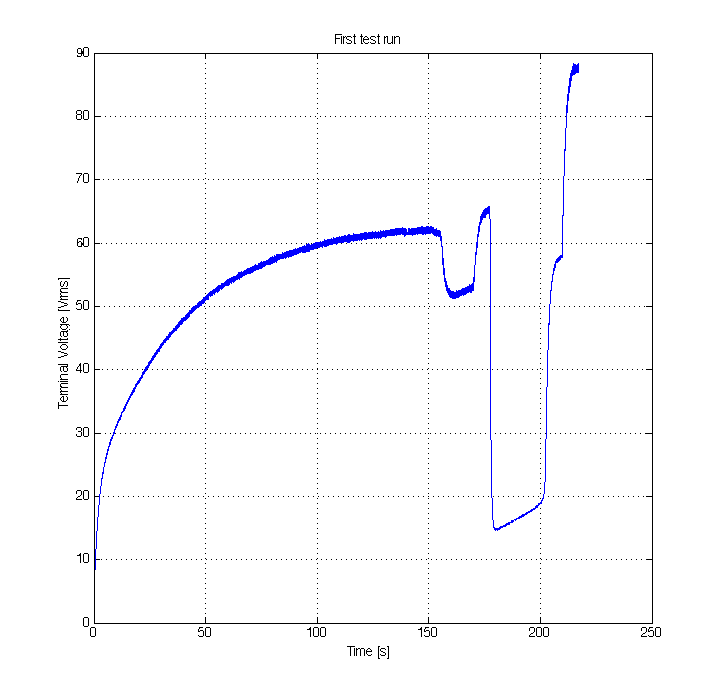
\includegraphics[scale=0.6]{./img/data_first.png}
\end{center}
\caption{Test results for the first test}
\label{fig:test1}
\end{figure}

Figure \ref{fig:final_test} shows the system response for the final test. The compensator used in this test was:
\begin{equation}
G_c(s) = \frac{s + 30}{s}
\end{equation}
Note the fast response time and relatively low overshoot.

\begin{figure}[h!]
\begin{center}
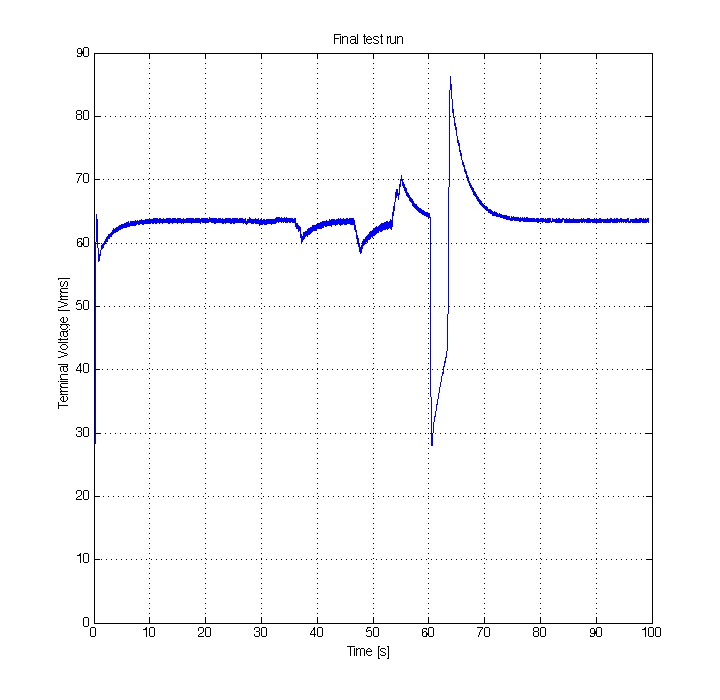
\includegraphics[scale=0.6]{./img/data_final.png}
\end{center}
\caption{Test results for the final test}
\label{fig:final_test}
\end{figure}



  \section{Conclusion}
The history and characteristics of power systems, especially synchronous generators, were discussed. The modeling, design, and testing phase were presented and documented. The proposed design proved to be superior to the other solutions presented as part of the in-class competition. The authors gained substantial knowledge about real-world compensator design used in power systems around the world.




% bibliography - using biblatex to include URLs
\newpage
\printbibliography[heading=bibintoc]

% the appendix, also optional
\newpage
\section*{Appendix}
\begin{appendices}

  \section{Appendix Test}
The variable \textit{bufferSize} contains the number of samples needed to archive the desired time duration. Recall the plot of the windowed signal in Figure \ref{fig:test_data} It is obvious that the spectrum analyzer would not display the spectrum of a signal correctly if it would take \textit{bufferSize} samples, perform spectral analysis, then take the next \textit{bufferSize} samples, perform spectral analysis and so on. The window function "pinches off" at the beginning and the end, which means that the information at signal components at the beginning and the end of the signal chunk would be lost.

I also want to test out the code feature: let's see how this works:
\lstinputlisting[caption=The \textit{process\_samples} function,style=customc,label=lst:process_samples]{./code/process_samples.c}

To counteract this effect, spectral analysis is performed on a window of \textit{bufferSize} samples, every time a new set of \textit{bufferSize/2} samples is acquired. This creates an overlapping effect and ensures that no information is lost due to windowing. Listing \ref{fig:sys} shows the relevant part of the \textit{process\_samples} function, where the circular buffer is filled and the samples for spectral analysis are prepared.


\end{appendices}
\end{document}
